%%%%%%%%%%%%%%%%%%%%%%%%%%%%%%%%%%%%%%%%%%%%%%%%%%%%%%%%%%%%%%%%%%%%%%%%
%
%		Chapter 3 - System Models
%
%%%%%%%%%%%%%%%%%%%%%%%%%%%%%%%%%%%%%%%%%%%%%%%%%%%%%%%%%%%%%%%%%%%%%%%%


\begin{topic}[Models of Systems]



\vfil

\begin{center}
\begin{minipage}{300pt}
	\includegraphics*[width=300pt]{images/chap3-xkcd.png}

	\hfill {\footnotesize (image from \href{https://www.xkcd.com/2063/}{xkcd - comic \#2063})}
\end{minipage}
\end{center}


\end{topic}






%%%%%%%%%%%%%%%%%%%%%%%%%%%%%%
%
%  MODULE - Modelling Two Interconnected Quantities
%
%%%%%%%%%%%%%%%%%%%%%%%%%%%%%%



\begin{module}{Modelling Two Quantities}
	\label{sys:model}

	In this module you will learn
\begin{itemize}
	\item how to model two or more inter-dependent quantities using systems
\end{itemize}

\hfill \\


Often, when modelling something, we are faced with two or more quantities that depend on each other. This means that one equation is not enough, so we need to learn how to deal with a system of equations. \\


Just like we did in module \ref{model-odes}, we will follow the step by step procedure developed in chapter 1.

\paragraph{\emph{Step 1.}} Define the problem

\begin{example}
We want to model two interacting populations, like the populations of bears and salmon in a specific natural park.\\

The first step is to decide on what we want to find at the end of the process. 
In this case, we want to know the number of individuals in each population and how they change as time passes. So we define:
\begin{itemize}
	\item $b(t) =$ number of bears in the natural park at time $t$;
	\item $s(t) =$ number of salmon in the natural park at time $t$.
\end{itemize}
\end{example}


\paragraph{\emph{Step 2.}} Build a mind map

\begin{example}
We start with both species in the centre:

\def\SalmonBear{
	\fill[color=orange!50!white] (-4,0) rectangle (-2,1) node[pos=.5] {\color{black}Salmon};
	\fill[color=brown!60!white] (4,0) rectangle (2,1) node[pos=.5] {\color{black}Bear};
}
\begin{center}
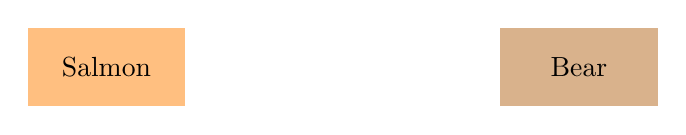
\begin{tikzpicture}
	\SalmonBear
\end{tikzpicture}
\end{center}

We can start brainstorming about the things that affect these populations:
\begin{center}
%\begin{tikzpicture}
%	\SalmonBear
%    \begin{scope}[decoration={
%    markings,
%    mark=at position 0.5 with {\arrow{>}}}
%    ]
%	\draw[postaction={decorate}] (-2,1) arc (120:60:4) node[pos=0.5,above] {food};
%    \draw[postaction={decorate}] (2,0) arc (300:240:4) node[pos=0.5,below] {hunts};
%    \end{scope}
%    \draw (-3,0) -- (-4,-1);
%    \fill[color=green!50!white] (-5.25,-2) rectangle (-2.75,-1) node[pos=.5] {\color{black}reproduction};
%    \draw (-3,1) -- (-4,2);
%    \fill[color=yellow!50!white] (-5.25,2) rectangle (-2.75,3) node[pos=.5] {\color{black}habitat limits};
%    \draw (3,0) -- (4,-1);
%    \fill[color=red!50!white] (5.25,-2) rectangle (2.75,-1) node[pos=.5] {\color{black}competition};
%    \draw (3,1) -- (4,2);
%    \fill[color=yellow!50!white] (5.25,2) rectangle (2.75,3) node[pos=.5] {\color{black}habitat limits};
%\end{tikzpicture}
\begin{tikzpicture}
	\SalmonBear
    \begin{scope}[decoration={
    markings,
    mark=at position 0.5 with {\arrow{>}}}
    ]
    \draw[postaction={decorate}] (-2,0.5) -- (2,0.5) node[pos=0.5,above] {food};
    \draw[postaction={decorate}] (2,0) arc (300:240:4) node[pos=0.5,below] {hunts};
    \end{scope}
    \draw (-3,0) -- (-4,-1);
    \fill[color=green!50!white] (-5.25,-2) rectangle (-2.75,-1) node[pos=.5] {\color{black}reproduction};
    \draw (-3,1) -- (-0.5,2);
    \draw (3,1) -- (0.5,2);
    \fill[color=yellow!50!white] (-1.5,2) rectangle (1.5,3) node[pos=.5] {\color{black}habitat limits};
    \draw (3,0) -- (4,-1);
    \fill[color=red!50!white] (5.25,-2) rectangle (2.75,-1) node[pos=.5] {\color{black}competition};
\end{tikzpicture}
\end{center}
	
\end{example}


\paragraph{\emph{Step 3.}} Make assumptions

\begin{example}
In this step, we discuss which of the boxes in the mind map we want to actually consider in our model, and which assumptions we need to make to consider them. \\

Let us start with how these species interact with each other:
\begin{enumerate}
	\item Salmon provide food for bears: the bear population profits from each encounter with salmon. How does each bear-salmon encounter affect the bear population?
	\item Bears hunt salmon: the salmon population is likely to decrease with each encounter with a bear. How does each bear-salmon encounter affect the salmon population?
\end{enumerate}

These two components are essential in our model, so we need to include them. It still leaves some freedom on how to do this. \\

There are other elements that we might want to include in our model:
\begin{enumerate}[start=3]
	\item Salmon reproduction: in the absence of predators and under ideal conditions, salmon should grow according to the Malthusian model, i.e. the rate of growth is proportional to the number of salmon;
	\item Bear competition: bears are mainly predators, so without salmon, their numbers will decrease, also according to the Malthusian model;
	\item Habitat limits: these species live in habitats that have limited resources, so we can consider a carrying capacity for each species.
\end{enumerate}

To make the model simpler, we will \emph{ignore habitat limits}. This means that this model will not be accurate if the populations become very large.
	
\end{example}


\paragraph{\emph{Step 4.}} Construct a model

\begin{example}
We will start with our populations:
\begin{itemize}
	\item $b(t)$
	\item $s(t)$
\end{itemize}
and we will start adding components to each of these one by one. \\

For the first two items, we need to estimate the number of encounters salmon-bear. We assume that the number of encounters is proportional to the number of all possible encounters: \emph{$b(t)\, s(t)$}.

\begin{enumerate}
	\item Salmon provide food for bears: for every possible salmon-bear encounter, there is a probability that a bear actually encounters a salmon, and then there is a chance that the bear will catch the salmon. Each catch improves the possibility that the bear population will increase. All these put together means that this factor should increase the bear growth rate by \emph{$a \,b(t)\, s(t)$}, where the constant $a$ needs to be found.
	\item Bears hunt salmon: similarly to the previous item, for every possible encounter, there is a probability that the bear actually encounters a salmon, and then there is a chance that the bear will catch the salmon. Every catch will decrease the salmon population, so the salmon growth rate will decrease by \emph{$c \,b(t) \,s(t)$}, there the constant $b$ needs to be found.
\end{enumerate}

Right now we have the following model:
$$
\begin{cases}
b'(t) = a \,b(t)\, s(t) + \cdots \\
s'(t) = - c \,b(t)\, s(t) + \cdots	
\end{cases}
$$

We continue with the other elements:
\begin{enumerate}[start=3]
	\item Salmon reproduction: this was explained before and should contribute to the salmon growth rate with the term \emph{$d s(t)$}.
	\item Bear competition: this was also explained above and should contribute to the bear growth rate with the term \emph{$-e b(t)$}.
	\item Habitat limits: we decided to ignore this.
\end{enumerate}

We have the model:
$$
\begin{cases}
b'(t) = a \, b(t) \,s(t) -e \, b(t) \\
s'(t) = - c \, b(t) \,s(t) + d \, s(t)
\end{cases}
$$

To find the constants $a,c,d,e$, we would probably need to go back to Step 3 and make further assumptions related to the way that we are measuring them.
\end{example}



\paragraph{\emph{Step 5.}} Model assessment

\begin{example}

We can do several things here. I'll let you brainstorm and think of ways you can assess this model.

One of the things that we can do is approximate its solutions using Euler's Method discussed in Module \ref{Approximation}. 

Let us assume, for this example the constants: $a=1$, $e=10$, $c=1$, $d=5$ and a time step $\Delta t = 0.5$ and we assumed an initial population of $b(0)=6$ and $s(0)=9$. Then we obtain the graph below:


\begin{center}
\includegraphics*[width=200pt]{images/module15-lotka-volterra.png}
\end{center}
\begin{itemize}
	\item \url{https://www.desmos.com/calculator/zywspwstwk} \hfill \qrcode{https://www.desmos.com/calculator/zywspwstwk}
\end{itemize}

The $x-$axis is the bear population while the $y-$axis is the salmon population. Each dot gives gives an approximation of the populations $\Delta t = 0.5$ time units after the previous approximation.\\


From this approximation, we can say infer that this model creates a population cycle, but it seems to spiral outwards: 
\begin{center}
\includegraphics*[width=200pt]{images/module15-lotka-volterra-more.png}
\end{center}

\begin{itemize}
	\item Is having a population cycle a feature that our model should have?
	\item Is the spiralling outwards a feature we want in our model?
	\item Is the spiralling a feature of the model or the approximation? If it's from the approximation, how does the model behave?
\end{itemize}

\end{example}

\begin{graybox}
Here is a GeoGebra approximation of the same model, called the Lotka-Volterra model:
\begin{itemize}
	\item \url{https://www.geogebra.org/m/KqNV7eHB} \hfill \qrcode{https://www.geogebra.org/m/KqNV7eHB}
\end{itemize}
\end{graybox}


\paragraph{\emph{Step 6.}} Putting it all together in a report

We'll skip this part here.





	\begin{exercises}

	\begin{problist}
	\prob Create a model for two competing populations, like cheetahs and lions: they don't hunt each other, but they hunt the same prey.
	
	\prob Create a model for two cooperating populations, like sharks and remoras. 

	\end{problist}
\end{exercises}

\end{module}



\begin{lesson}
	\Title{Modelling Two Quantities}

	\Heading{Objectives}
	\begin{itemize}
		\item Bla
	\end{itemize}
	
	\Heading{Motivation} 

\end{lesson}




\newpage

\question We want to model two competing populations, like cheetahs and lions: they don't hunt each other, but they hunt the same prey.
\begin{parts}
	\item Create a model for these two populations.
	\item Using Desmos or WolframAlpha, create a slope field in the plane where the horizontal axis is one population and the vertical one is the other.
	\item Using the slope field, deduce some properties of your model and discuss how closely it matches what you expect from these populations.

	\item Extend the model to include a population of antelopes.	
\end{parts}





\bookonlynewpage


\question
	A cheetah is chasing an antelope. We want a model of their positions as they run.
	
	
\begin{annotation}
	\begin{goals}
		This exercise is not required to do in lecture.
		
		Allow some brainstorming and try to create a structure for this problem:
		\begin{itemize}
			\item Positions seen from above ($xy-$plane).
			\item Only need $x_a(t), y_a(t)$ and $x_c(t), y_c(t)$
			\item Focus on the cheetah: where is she heading to?
			\item For the antelope, students need to come up with an escape strategy
			\item Model will be nonlinear!
		\end{itemize}
	\end{goals}
\end{annotation}





%%%%%%%%%%%%%%%%%%%%%%%%%%%%%%
%
%  MODULE - Solving Systems
%
%%%%%%%%%%%%%%%%%%%%%%%%%%%%%%



\begin{module}{Systems of two linear ODEs with constant coefficients}
	\label{sys:solve}

	In this module you will learn
\begin{itemize}
	\item how to solve systems of two linear first-order ODEs with constant coefficients
\end{itemize}

\hfill \\


First, a system of two first-order ODEs has the form:
$$
\begin{cases}
x'(t) = f\big(t, x(t),y(t)\big) \\	
y'(t) = g\big(t, x(t),y(t)\big)
\end{cases}
$$
where the functions $f$ and $g$ are continuous and have continuous derivatives. \\

This system could be nonlinear, so we are only considering linear systems with constant coefficients, which means that they have a very specific form:
$$
\begin{cases}
	x'(t) = a x(t) + b y(t) + e\\
	y'(t) = c x(t) + d y(t) + f
\end{cases}
%
\quad \Leftrightarrow \quad 
	\begin{bmatrix} x'(t) \\ y'(t) \end{bmatrix}
	=
	\begin{bmatrix} a & b \\ c & d \end{bmatrix}
	\begin{bmatrix} x(t) \\ y(t) \end{bmatrix}
	+	\begin{bmatrix} e \\ f \end{bmatrix}
%
\quad \Leftrightarrow \quad 
	\vec{r}'(t)
	=
	A \, \vec{r}(t) + \vec{b}
$$
where
$$
\vec{r}(t) = \begin{bmatrix} x(t) \\ y(t) \end{bmatrix}
\quad , \quad 
A = \begin{bmatrix} a & b \\ c & d \end{bmatrix}
\quad and \quad 
\vec{b}=\begin{bmatrix} e \\ f \end{bmatrix}.
$$

The unknown functions we are trying to find is $\vec{r}(t)$. \\


\paragraph{\emph{Homogeneous Systems.}} These are systems of the form above with $\vec{b} = \vec{0}$.

This means that we want to find all functions $\vec{r}(t)$ that satisfy
$$
\vec{r}'(t) = A \vec{r}(t).
$$


\begin{example}
Let us start with an example of the same problem where $\vec{r}(t)$ is a ``one-dimensional'' vector, a scalar function $u(t)$, and the matrix $A$ is a ``one-dimensional matrix'', a constant $a$. \\

We want to solve the problem	
$$
u'(t) = a \cdot u(t).
$$

We have seen how to solve these kind of problems before. The solutions are
$$
u(t) = c e^{at},
$$
where $c$ can be any constant.
\end{example}

In our two-dimensional case, it is a little more complicated. We can't just write $e^{At}$ where $A$ is a matrix (this expression can make sense, but we would have to find out what is the exponential of a matrix). \\

So we can use the example above to make an \emph{educated guess}: the solution should look like an exponential:
$$
\vec{r}(t) = 
\vec{c} \, e^{\lambda t},
$$
where $\vec{c}$ is a constant vector. \\

If our guess is correct, to find $\vec{r}(t)$, we only need to find $\lambda$ and $\vec{c}$. \\

Let us see what happens when we use this guess and plug it into the system of ODEs:
\begin{align*}
\vec{r}'(t) = A \vec{r}(t) \quad
	& \Leftrightarrow \quad \vec{c} \lambda e^{\lambda t} = A \vec{c} e^{\lambda t} \\
	& \Leftrightarrow \quad \vec{c} \lambda = A \vec{c}.
\end{align*}

This is a problem you have seen before -- and eigenvalue-eigenvector problem: 
\begin{itemize}
	\item $\lambda$ can be any eigenvalue of the matrix $A$
	\item $\vec{c}$ can be any eigenvector of $A$ associated with $\lambda$ 
\end{itemize}

This means that we might have multiple choices for eigenvalues and eigenvectors, or even that eigenvalues and eigenvectors involve complex numbers.
Let us split our study of possible solutions in three cases.



%%%%%%%%%       %%%%%%%%%       %%%%%%%%%       %%%%%%%%%       %%%%%%%%%

\subsection{Two real and distinct eigenvalues}

\begin{example}
Consider the problem
$$
\vec{r}'(t) = \begin{bmatrix}	
 10 & 18 \\ -6 & -11	
 \end{bmatrix} \, \vec{r}(t).
$$

Then, the eigenvalues and eigenvectors of the matrix are
\begin{itemize}
	\item $\lambda_1=-2$ with eigenvector $\vec{v}_1 = \begin{bmatrix} 3 \\ -2 \end{bmatrix}$
	\item $\lambda_2=1$ with eigenvector $\vec{v}_2 = \begin{bmatrix} 2 \\ -1 \end{bmatrix}$
\end{itemize}

This means that we found two solutions:
$$
\vec{r}_1(t) = \begin{bmatrix} 3 \\ -2 \end{bmatrix} e^{-2t}
\quad \text{ and } \quad \vec{r_2}(t) = \begin{bmatrix} 2 \\ -1 \end{bmatrix} e^{t}.
$$

Then, we can show that 
$$
\vec{r}(t) = c_1 \begin{bmatrix} 3 \\ -2 \end{bmatrix} e^{-2t}
+c_2\begin{bmatrix} 2 \\ -1 \end{bmatrix} e^{t}
$$
is also a solution of the problem for any constants $c_1$ and $c_2$.

In fact, we can show that this formula captures all possible solutions for this problem.
\end{example}


\begin{video}
	\begin{itemize}
		\item \qrvideo{https://youtu.be/YUjdyKhWt6E}
	\end{itemize}
\end{video}




%%%%%%%%%       %%%%%%%%%       %%%%%%%%%       %%%%%%%%%       %%%%%%%%%

\subsection{Two complex eigenvalues}

We actually don't need to know a lot about complex numbers to be able to understand how to solve this case.
The results about complex values that are necessary to know will be included in the box below.

\begin{definition}[Complex numbers]
\begin{itemize}
	\item A complex number is a number of the form $z=a+ib$ where $i$ is called the imaginary constant and satisfies $i^2=-1$.
	\item Given a complex number $z=a+ib$, we call $\overline{z}=a-ib$ its complex conjugate. It satisfies:
	$$ z \cdot \overline{z} = a^2+b^2 = |z|^2.$$

	\item If a matrix has real components and two complex eigenvalues, then the eigenvalues are complex conjugates of each other. Moreover, the eigenvectors are also complex conjugates of each other.
	\item Euler's Formula: $e^{i \theta} = \cos(\theta) + i \sin (\theta)$.
\end{itemize}
\end{definition}




\begin{example}
Consider the problem
$$
\vec{r}'(t) = \begin{bmatrix}	
 1 & 1 \\ -1 & 1
 \end{bmatrix} \, \vec{r}(t).
$$

Then, the eigenvalues and eigenvectors of the matrix are
\begin{itemize}
	\item $\lambda_1=1+i$ with eigenvector $\vec{v}_1 = \begin{bmatrix} -i \\ 1 \end{bmatrix}$
	\item $\lambda_2=1-i$ with eigenvector $\vec{v}_2 = \begin{bmatrix} i \\ 1 \end{bmatrix}$
\end{itemize}

This means that we found two solutions:
$$
\vec{r}_1(t) = \begin{bmatrix} -i \\ 1 \end{bmatrix} e^{(1+i)t}
\quad \text{ and } \quad \vec{r}_2(t) = \begin{bmatrix} i \\ 1 \end{bmatrix} e^{(1-i)t}.
$$

Then, all solutions of this system of ODEs can be expressed as
$$
\vec{r}(t) = c_1 \begin{bmatrix} -i \\ 1 \end{bmatrix} e^{(1+i)t}
+c_2\begin{bmatrix} i \\ 1 \end{bmatrix} e^{(1-i)t}.
$$

There is a problem with the form of these solutions: they involve complex numbers!

Imagine that we start with a problem where we have two (real) quantities that interact with each other through this system of differential equations.
Then we expect these quantities to measure in real numbers, not complex.

\begin{itemize}
	\item This means that we expect \emph{the imaginary part of this solutions to cancel out}.
\end{itemize}

So let us manipulate this formula using Euler's formula and see if we can re-write in such a way that doesn't involve complex numbers. \\

We have:
\begin{align*}
	e^{(1+i)t} &= e^t \cdot e^{it} = e^t \big( \cos(t) + i \sin(t)\big) \\
	e^{(1-i)t} &= e^t \cdot e^{-it} = e^t \big( \cos(t) - i \sin(t)\big)
\end{align*}

So our solution expands to:
$$
\vec{r}(t) = c_1 \begin{bmatrix} -i \\ 1 \end{bmatrix} e^t \big( \cos(t) + i \sin(t)\big)
+c_2\begin{bmatrix} i \\ 1 \end{bmatrix} e^t \big( \cos(t) - i \sin(t)\big).
$$

We can now manipulate this expression:
\begin{align*}
\vec{r}(t) 
	& = e^t
		\begin{bmatrix}
			-i c_1 	\big( \cos(t) + i \sin(t)\big) + i c_2 \big( \cos(t) - i \sin(t)\big) \\
			c_1 	\big( \cos(t) + i \sin(t)\big) + c_2 \big( \cos(t) - i \sin(t)\big) \\
		\end{bmatrix} \\
	& = e^t 
		\begin{bmatrix}
			(c_1+c_2) \sin(t) - i (c_1-c_2) \cos(t) \\
			(c_1+c_2) \cos(t) + i(c_1-c_2) \sin(t)
		\end{bmatrix} \\
	& = e^t \left( (c_1+c_2) \begin{bmatrix} \sin(t) \\ \cos(t) \end{bmatrix}
		+ i (c_1 -c_2) \begin{bmatrix} - \cos(t) \\ \sin(t) \end{bmatrix}
		\right)
\end{align*}

So now we do something that might look like a ``cheating''. We define:
$$
a_1 = c_1+c_2 \quad \text{ and } \quad a_2 = i (c_1-c_2).
$$


Then the solution is
$$
\vec{r}(t) = a_1\begin{bmatrix} \sin(t) \\ \cos(t) \end{bmatrix} e^t
		+ a_2 \begin{bmatrix} - \cos(t) \\ \sin(t) \end{bmatrix} e^t.
$$

This last form doesn't include any complex numbers and is equivalent to the previous form.

\end{example}

\begin{graybox}
	It may look like the final solution above still includes complex numbers in the constants $a_1$ and $a_2$. 
	
	To convince yourself that this is not the case, solve the following exercise.\\
	
	Find the unique solution of
	$$
	\vec{r}'(t) = \begin{bmatrix}	
 		1 & 1 \\ -1 & 1
		\end{bmatrix} 
		\, \vec{r}(t)
	\qquad \text{ with} \qquad
	\vec{r}(0) = \begin{bmatrix}
 			-3 \\ 2
	 \end{bmatrix}
	 $$
	 
	 Find the constants $c_1, c_2$ and then the constants $a_1,a_2$. Which ones are complex and which ones are real?
\end{graybox}

\begin{video}
	\begin{itemize}
		\item \qrvideo{https://youtu.be/TRVS5Wo9LoM}
	\end{itemize}
\end{video}



%%%%%%%%%       %%%%%%%%%       %%%%%%%%%       %%%%%%%%%       %%%%%%%%%

\subsection{One repeated real eigenvalue}


\begin{example}
Consider the problem
$$
\vec{r}'(t) = \begin{bmatrix}	
 5 & 0 \\ 1 & 5	
 \end{bmatrix} \, \vec{r}(t).
$$

Then, there is only one eigenvalue with one eigenvector
\begin{itemize}
	\item $\lambda_1=5$ with eigenvector $\vec{v}_1 = \begin{bmatrix} 0 \\ 1 \end{bmatrix}$, which yield a solution $\vec{r}_1(t) = c_1 \begin{bmatrix} 0 \\ 1 \end{bmatrix} e^{5t}$.
\end{itemize}

This is a \emph{problem} because we need two solutions to put together and obtain two constants, as in the two previous cases.
%\end{example}

\begin{graybox}
To convince yourself that it is a problem, try solving the problem above with initial conditions
$$
\vec{r}(0) = \begin{bmatrix}	0 \\ 4 \end{bmatrix}.
$$

What about with initial conditions
$$
\vec{r}(0) = \begin{bmatrix}	 1 \\ 4 \end{bmatrix} \quad ?
$$
\end{graybox}

%\begin{example}

This means that we ware missing one solution -- that will enable us to solve the problem for any initial conditions. \\


Let us re-write the original problem in a different form by letting 
$$
\vec{r}(t) = \begin{bmatrix} x(t) \\ y(t)\end{bmatrix}.
$$
Then we have
$$
\begin{cases}
x'(t) = 5 x(t) \\
y'(t) = x(t) +5 y(t)	
\end{cases}
$$
These are two ODEs, but we can solve the first and then tackle the second one.
We obtain
$$
\begin{cases}
	x(t) = c_2 e^{5t} \\
	y(t) = 	c_1 e^{5t} + c_2 t e^{5t} 
\end{cases}
\quad \Leftrightarrow \quad
	\vec{r}(t) = \begin{bmatrix}
		c_2 \\ c_1 + c_2 t
	\end{bmatrix} e^{5t}
\quad \Leftrightarrow \quad
	\vec{r}(t) = c_1 \begin{bmatrix} 0 \\ 1 \end{bmatrix} e^{5t} + c_2
	\begin{bmatrix}	1 \\ t
	\end{bmatrix} e^{5t}
$$
\end{example}

\begin{graybox}
Observe that the solution we found has the form:
$$
	\vec{r}(t) = \underbrace{c_1 \begin{bmatrix} 0 \\ 1 \end{bmatrix} e^{5t}}_{\text{solution } \vec{r}_1(t)} + c_2 \left( 
	\underbrace{\begin{bmatrix}	1 \\ 0 \end{bmatrix}}_{\text{new vector } \vec{w}} e^{5t} + \underbrace{\begin{bmatrix} 0  \\ 1 
	\end{bmatrix}}_{\vec{v}_1} t e^{5t}\right).
$$

So we can make another \emph{educated guess} that the solution we were missing has the form:
$$
\vec{r}_2(t) = \left(\vec{w} + \vec{v}_1 t\right) e^{\lambda t}.
$$

With this form in mind, we can plug it into the system of ODEs \quad $\vec{r}'(t) = A \vec{r}(t)$ \quad, which has exactly one eigenvalue $\lambda$, to get:
$$
\lambda \vec{w}e^{\lambda t} + \lambda \vec{v}_1 t e^{\lambda t} + \vec{v}_1 e^{\lambda t}
= A \vec{w} e^{\lambda t} + A \vec{v}_1 t  e^{\lambda t}
$$
which is equivalent to:
$$
\lambda \vec{w} + \underbrace{\lambda \vec{v}_1}_{=A \vec{v}_1} t  + \vec{v}_1
= A \vec{w}  + A \vec{v}_1 t 
	\quad \Leftrightarrow \quad
	\left( \lambda I - A \right ) \vec{w} = \vec{v}_1
$$
%which becomes
%$$
%\lambda \vec{w} + \vec{v}_1
%= A \vec{w}  
%	\quad \Leftrightarrow \quad
%	\left( \lambda I - A \right ) \vec{w} = \vec{v}_1
%$$

Since at this point we already know $\lambda$ and $\vec{v}_1$, we can now find $\vec{w}$ in a similar way used to find the eigenvector $\vec{v}_1$. The vector $\vec{w}$ is called a \emph{generalized eigenvector} of $A$ associated with the eigenvalue $\lambda$.

\end{graybox}

\begin{video}
	\begin{itemize}
		\item \qrvideo{https://youtu.be/hCShTLmeZN4}
	\end{itemize}
\end{video}






	\input{modules/module16-sys-solving-exercises.tex}
\end{module}



\begin{lesson}
	\Title{Systems of two linear ODEs with constant coefficients}

	\Heading{Objectives}
	\begin{itemize}
		\item Bla
	\end{itemize}
	
	\Heading{Motivation} 

\end{lesson}




\newpage

\question
Consider a cheetah-lion inspired problem:
$$
\frac{d \,\vec{r}}{dt} = \begin{bmatrix} 3 & -2 \\ -1 & 4\end{bmatrix} \vec{r}.
$$
	
\begin{parts}
	\item Find the two solutions $\vec{r}_1, \vec{r}_2$.
	\item Is $\vec{r}_1(t) + \vec{r}_2(t)$ a solution?
	\item Is $\vec{r}_1(t) - \vec{r}_2(t)$ a solution?
	\item Is $2\vec{r}_1(t) + 3\vec{r}_2(t)$ a solution?
	\item What is the general solution?
	\item Find the solution that satisfies $\vec{r}(0) = \begin{bmatrix} 6 \\ 7\end{bmatrix}$?
\end{parts}


\bookonlynewpage


\question
Consider a problem:
$$
\frac{d \,\vec{r}}{dt} = \begin{bmatrix} 2 & -5 \\ 1 & -2\end{bmatrix} \vec{r}.
$$
	
\begin{parts}
	\item Find the general solution.
	\item Find the solution that satisfies $\vec{r}(0) = \begin{bmatrix} 6 \\ 7\end{bmatrix}$?
\end{parts}




\bookonlynewpage


\question
Consider a problem:
$$
\frac{d \,\vec{r}}{dt} = \begin{bmatrix} 4 & -1 \\ 8 & -2\end{bmatrix} \vec{r} - \begin{bmatrix} 5 \\ 10 \end{bmatrix}.
$$
%[2,3]
\begin{parts}
	\item Find the equilibrium solution.
	\item Find the general solution.
	\item Find the solution that satisfies $\vec{r}(0) = \begin{bmatrix} 2 \\ 3\end{bmatrix}$?
\end{parts}








%%%%%%%%%%%%%%%%%%%%%%%%%%%%%%
%
%  MODULE - Phase Portraits
%
%%%%%%%%%%%%%%%%%%%%%%%%%%%%%%



\begin{module}{Phase Portraits}
	\label{sys:phase}

	In this module you will learn
\begin{itemize}
	\item how to sketch a phase portrait for a linear system of ODEs with constant coefficients
	\item how to use a phase portrait to deduce properties of solutions
\end{itemize}

\hfill \\

When we solve a system of two ODEs, we obtain two functions $x(t)$ and $y(t)$, so when we want to graph solutions, we have a problem:
\begin{itemize}
	\item Should we sketch each of these functions separately?
	\item Should we sketch them together?
	\item Should we sketch the path as if a particle is moving with coordinates $x(t)$ and $y(t)$?
\end{itemize}

\begin{example}
Consider the initial-value problem
$$
\frac{d\,\vec{r}}{dt} = \begin{bmatrix} 0 & 1 \\ -1 & 0 \end{bmatrix}\vec{r} \quad \text{ with } \quad \vec{r}(0)=\begin{bmatrix} 0 \\ 1 \end{bmatrix},
$$
which has the solution
$$
\vec{r}(t) = \begin{bmatrix}
	\sin(t) \\ \cos(t)
\end{bmatrix}.
$$

Which of the following ways are better?
\begin{itemize}
\item \begin{minipage}{400pt}\includegraphics[width=400pt]{images/module17-sep-xy.pdf}\end{minipage}

\item \begin{minipage}{200pt}\includegraphics*[width=200pt]{images/module17-together-xy.pdf}\end{minipage}

\item \begin{minipage}{200pt}\includegraphics[height=200pt]{images/module17-phaseportrait.pdf}\end{minipage}
\end{itemize}

There is no correct answer, but the last graph gives more information on how the two quantities interact with each other, so we will focus on that type of graph.
\end{example}


The graphs in the example above are graphs of one specific solution. A phase portrait gives an idea of all possible solutions. 
\begin{example}
The last graph of the example is part of which phase portrait?

\begin{center}
\includegraphics*[width=420pt]{images/module17-possiblephaseportraits.pdf}
\end{center}

A phase portrait gives a good idea of how all solutions behave.
\end{example}

Sketching phase portraits for systems of two first-order linear ODEs is important because it gives us insight on how the two components affect each other for all solutions.

\begin{example}
Consider the problem
$$
\frac{d \, \vec{r}}{dt} = \begin{bmatrix} -2 & 3 \\ -3 & -2 \end{bmatrix} \vec{r},
$$
where the matrix $A$ has the eigenvalues and eigenvectors:
\begin{itemize}
	\item Eigenvalues $\lambda_{\pm} = -2 \pm 3i$ with eigenvectors $v_{\pm} = \begin{bmatrix} \mp i \\ 1 \end{bmatrix}$
\end{itemize}

This means that the general solution has the form
\begin{itemize}
	\item $\displaystyle \vec{r}(t) = a_1 \begin{bmatrix} -i \\ 1 \end{bmatrix} e^{(-2+3i)t} + a_2 \begin{bmatrix} i \\ 1 \end{bmatrix} e^{(-2-3i)t}$

	\item[or]
	\item $\displaystyle \vec{r}(t) = c_1 \begin{bmatrix}	 \sin(3t) \\ \cos(3t) \end{bmatrix} e^{-2t} + c_2 \begin{bmatrix}	 -\cos(3t) \\ \sin(3t) \end{bmatrix} e^{-2t}$ \\
\end{itemize}

We can use the general form and start sketching some solutions.

\begin{itemize}
	\item Let $c_1=1$ and $c_2=0$ and we obtain
	$$ \vec{r}(t) = \begin{bmatrix}	 \sin(3t) \\ \cos(3t) \end{bmatrix} e^{-2t}.$$
	
	To sketch this solution, let us start by ignoring the term $e^{-2t}$. 
	
	So we want to sketch $ \vec{r}(t) = \begin{bmatrix}	 \sin(3t) \\ \cos(3t) \end{bmatrix}$:
	\begin{center}
		\includegraphics[height=200pt]{images/module17-phaseportrait.pdf}
	\end{center}
	
	The path is going in circles in the clockwise direction.
	
	By multiplying the solution by $e^{-2t}$, which starts at $1$ when $t=0$ and keeps decreasing towards $0$ as $t$ increases, we are creating a graph that keeps revolving around the origin as it converges towards the origin, yielding a spiral.
	\begin{center}
		\includegraphics[height=200pt]{images/module17-spiral.pdf}
	\end{center}
	
	In this graph, we also include the graph for $t<0$. \\
	
	\item Let $c_1=-1$ and $c_2=0$ and we obtain
	$$ \vec{r}(t) = \begin{bmatrix}	 -\sin(3t) \\ -\cos(3t) \end{bmatrix} e^{-2t}$$	
	
	We add this graph to the previous one.
	\begin{center}
		\includegraphics[height=200pt]{images/module17-spiral2.pdf}
	\end{center}
	
	\item Let $c_1=0$ and $c_2=\pm 1$ and we obtain
	$$ \vec{r}(t) = \begin{bmatrix}	 \mp \cos(3t) \\ \pm\sin(3t) \end{bmatrix} e^{-2t}.$$

	And add these to the graph:
	\begin{center}
		\includegraphics[height=200pt]{images/module17-spiral3.pdf}
	\end{center}

\end{itemize}

Sometimes, we need some solutions of the type $c_1=\pm 1$ and $c_2=\pm 1$ to get some different types of solutions, but we'll let you discover that on the core exercises.

These four solutions seem to give a good idea of all possible solutions: clockwise spirals converging to the origin.\\


Also observe that $\vec{r}(t) = \begin{bmatrix}0 \\ 0\end{bmatrix}$, so this system has an equilibrium solution.

This kind of equilibrium is called a \emph{spiral sink} and it is \emph{asymptotically stable}.
This means that it is a spiral and it converges to the equilibrium (the origin).
\end{example}





\begin{video}
	\begin{itemize}
		\item \qrvideo{https://youtu.be/nyI_JPDrJ_I}
		\item \qrvideo{https://youtu.be/dpbRUQ-5YWc}
	\end{itemize}
\end{video}





	\input{modules/module17-sys-phase-exercises.tex}
\end{module}



\begin{lesson}
	\Title{Phase Portraits}

	\Heading{Objectives}
	\begin{itemize}
		\item Bla
	\end{itemize}
	
	\Heading{Motivation} 

\end{lesson}




\newpage

\question
	Core Exercise with several parts
\begin{parts}
	\item Part 1
	\item Part 2
\end{parts}


\bookonlynewpage


\question
	One more core exercise



